\documentclass[12pd]{article}
\usepackage[utf8]{inputenc}
\usepackage[T2A]{fontenc}
\usepackage[mongolian]{babel} 
\usepackage{graphicx}
\graphicspath{{images/}}
\begin{document}
	\section{Функциональ шаардлага}
	\begin{itemize}
		\item Багш
		\item Цагийн тооцоо гаргана 
		\item Ажилд ирсэн цагаа тооцно 
		\item Хэвтээ босоо хүснэгт бөглөнө 
		\item Цагийн тооцоогоо баталгаажуулна 
		\item Алдаатай цагийн тооцоог засна(Edit and Delete)
		\item Тэнхимийн эрхлэгч 
		\item Цагийн тооцоог хянах 
		\item Алдаатай цагийн тооцоог comment хэсэгт бичнэ
		\item Цагийн тооцоог устгана 
		\item Сургалтийн алба 
		\item Илүү цагийн тооцоо гаргана
		
		
		
		
		
		
	\end{itemize}
	\section{Функциональ бус шаардлга}
	\begin{itemize}
		\item 
		\item
		\item
	\end{itemize}
	\section{Usecase diagram}
	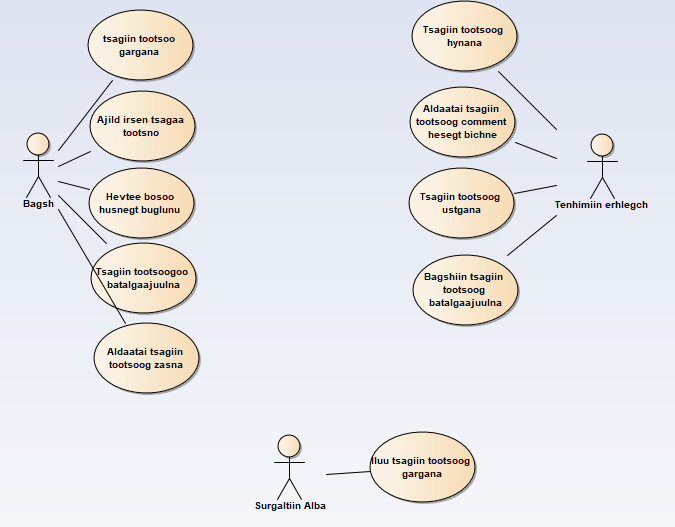
\includegraphics[width=\textwidth]{usecase}
	\section{Цаг бүртгэлийн дэлгэц}
	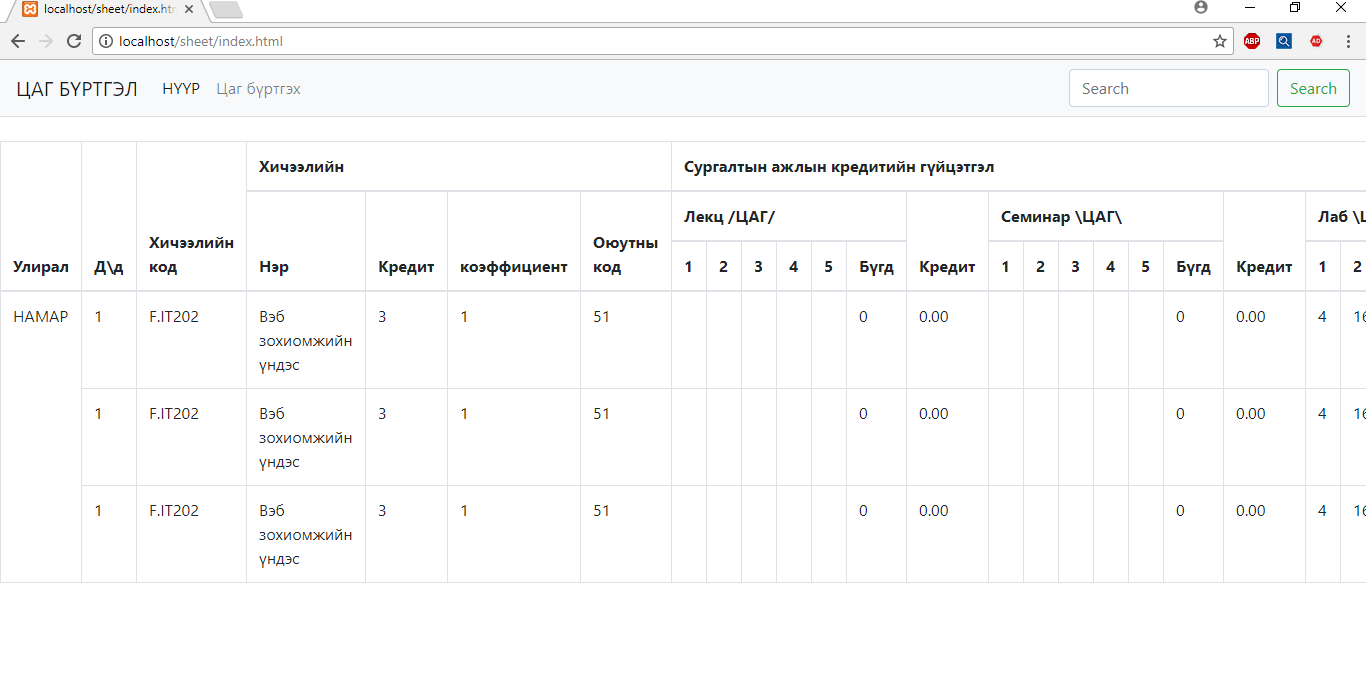
\includegraphics[width=\textwidth]{delgets1}
	\section{Цаг бүртгэлийн дэлгэц}
	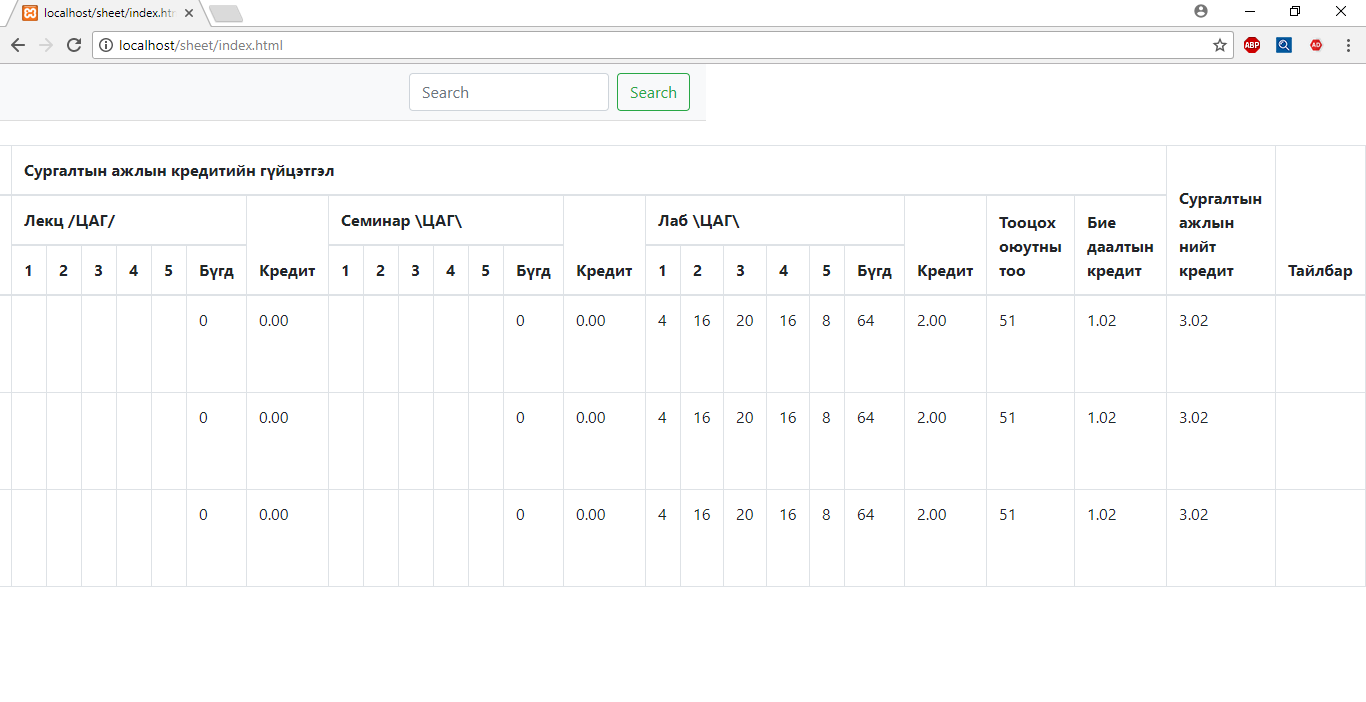
\includegraphics[width=\textwidth]{delgets2}
	\section{Цаг бүртгэлийн дэлгэц}
	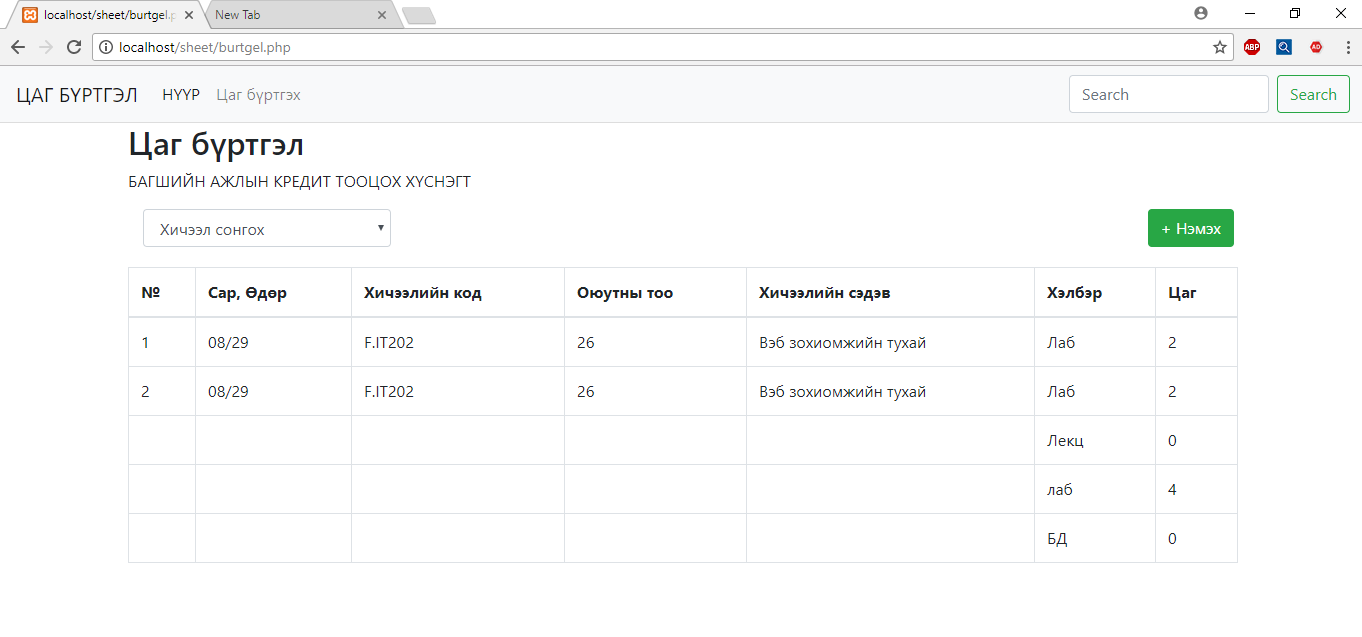
\includegraphics[width=\textwidth]{delgets3}
	\section{ERD}
	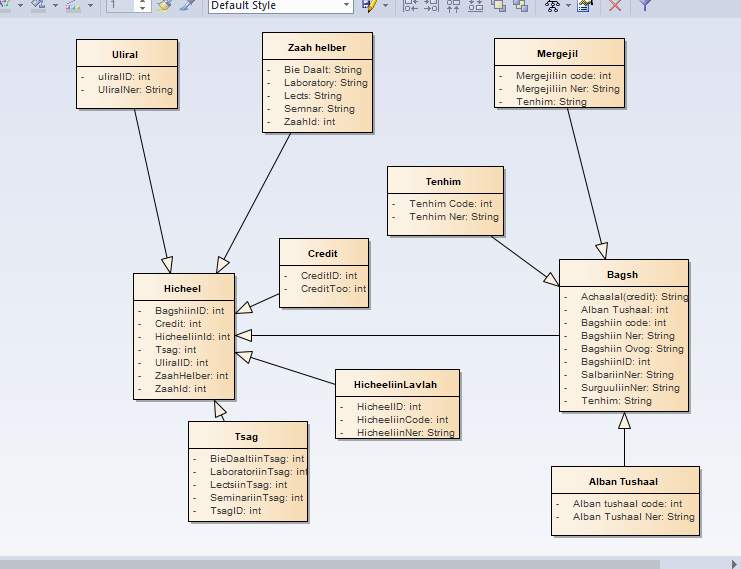
\includegraphics[width=\textwidth]{ERD}
	
	\section{Activity diagram}
	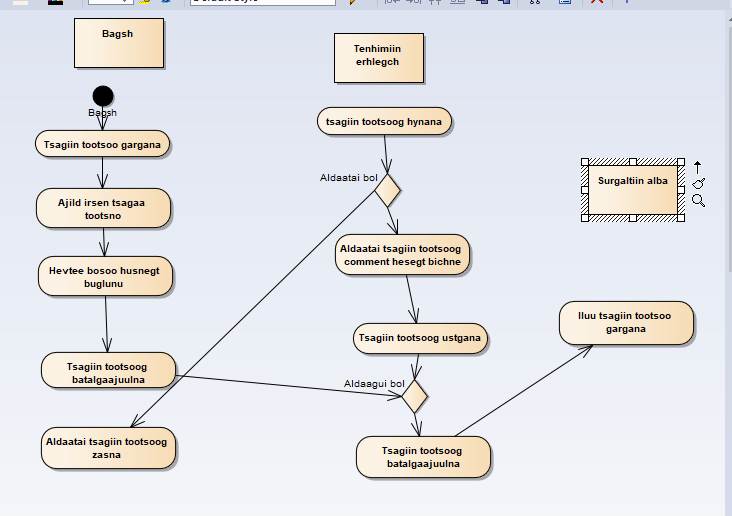
\includegraphics[width=\textwidth]{Activity}
	\section{Class diagram}
	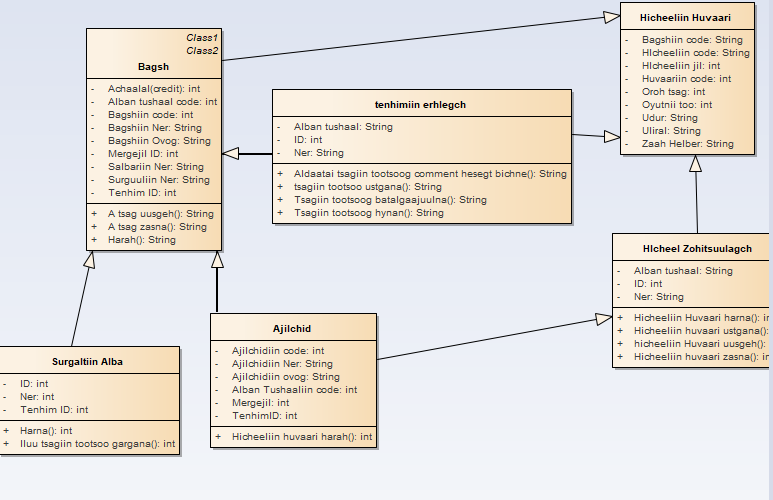
\includegraphics[width=\textwidth]{CD}
	\section{Sequence  diagram}
	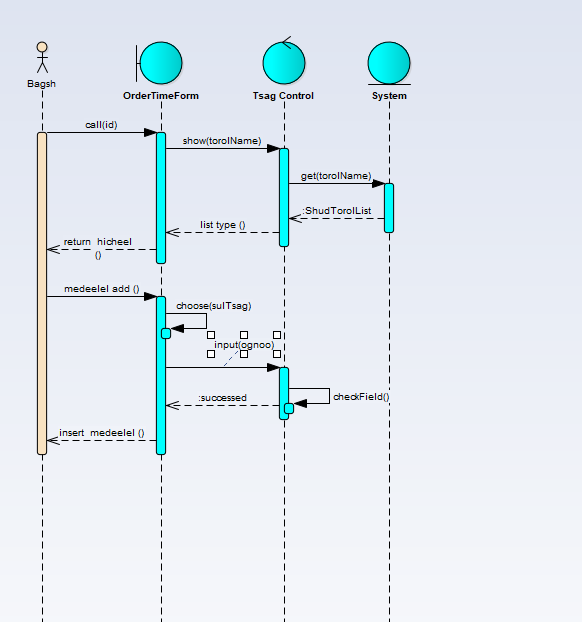
\includegraphics[width=\textwidth]{sequence}
	
	
	
	
	
	
\end{document}



